\renewcommand\categorylabel{[PROJEKT.EINBLICK]}

\renewcommand\authorsline{Vorname Nachname, Vorname Nachname, Vorname Nachname, ...}

\stylesectionMC{Mensch-Maschine-Interaktion im virtuellen Raum erproben: Der Fahrsimulator des KIT-IFAB\label{sec:ifab}}{Die Interaktion zwischen Mensch und Fahrzeug spielt eine zentrale Rolle -- in Bezug auf Sicherheit, Komfort und Effizienz. Das hat auch der technische Fortschritt durch neue Mobilitätslösungen nicht geändert, im Gegenteil: Durch Automatisierung und neue Interaktionskonzepte ist das Zusammenspiel wesentlich komplexer geworden. Um Assistenzsysteme und automatisierte Fahrfunktionen zu entwickeln, in denen die Insassen mitgedacht sind, Institut für Arbeitswissenschaft und Betriebsorganisation (IFAB) am KIT einen Fahrsimulator, der umfangreiche Probandenstudien ermöglicht. Wir werfen einen Blick vor Ort auf die Technik und die damit verbundenen Möglichkeiten.
\vspace{-10pt}% <- Das vspace ist für das konkrete Layout mit dem Hintergrundbild nötig, das kann je nachdem auch entfallen.
}
{% Was in diesen Klammern steht, wird am Anfang der Seite ausgeführt. Wenn ihr alles hier drin auskommentiert erhaltet ihr einen "normalen" Beitrags-Anfang.
\vspace{5.5cm} % Verschieben der Überschrift
\replaceSSColor{white}% Wenn man diese Zeile auskommentiert, sind die Titeltexte dunkelblau und grün (ihre Normalwerte), für den schwarzen Hintergrund werden sie hier in diesem Beitrag auf weiß gesetzt.
\ThisULCornerWallPaper{1.007}{content/caudri/images/ifab1c}% Hintergrundbild
\pagecolor{white} % Farbseite
}




\afterpage{%
\resetSSColor
}

// Hier kommt unser Artikel rein:

\section{Allgemein}
Im Allgemeinen ist die CAuDri-Challenge ein studentischer Hochschulwettbewerb, bei dem verschiedene
ehrenamtliche Gruppen von unterschiedlichen Hochschulen zusammenkommen. Der Wettbewerb wurde letztes Jahr 2023
zum ersten Mal in Stuttgart ausgetragen. Die Hochschulgruppen entwickeln in Ihrer Freizeit ein autonom Fahrendes
Modellfahrzeug im Maßstab 1:10 und treten an der Challenge in zwei verschiedenen Disziplinen gegeneinander an.

\section{Disziplinen} 
Während des gesamten Events wird die Performance der Modellfahrzeuge in zwei unterschiedlichen
Disziplinen auf die Probe gestellt und währenddessen von Schiedsrichtern bewertet. Die erste Disziplin ist der
„Freedrive“, wo das Fahrzeug in einer vorgegebenen Zeit so viele Streckenmeter wie möglich zurücklegen
muss. Die zweite Disziplin bezeichnet sich als „Obstacle Evasion“. Hier wird die Strecke um zusätzliche
Hindernisse erweitert, welche beim Fahren berücksichtigt werden müssen.

Wie bereits erwähnt wird die Performance des Fahrzeugs von Schiedsrichtern bewertet. Für jede Disziplin wird
eine bestimmte Anzahl von Punkten vergeben, welche sich aus verschiedenen Faktoren wie zum Beispiel der insgesamt
zurückgelegten Strecke und das erfolgreiche Passieren unterschiedlicher Hindernisse. Werden Regularien verletzt,
werden entsprechend Punkte abgezogen.  

\subsection{Freedrive} Die „Freedrive-Disziplin“ dient dazu die allgemeine
Fahrsituation eines außerörtlichen Fahrszenarios zu simulieren. Auf der gesamten ausgelegten Fahrstrecke befinden
sich demnach keine Hindernisse. Das Fahrzeug muss während dem Abfahren der Strecke nur Straßenkreuzungen beachten
und die entsprechenden Fahrbahnmarkierungen nicht überfahren.

Wie bereits oben erläutert wird in dieser Disziplin die Schnelligkeit des Fahrzeugs in Bezug auf die zurückgelegte
Strecke nach einer bestimmten Zeit bewertet. Bei der „Freedrive-Disziplin“ wird gleichzeitig das Parken
simuliert. Dazu werden an einer bestimmten Stelle verschiedene Parkbuchten eingebaut. Einige der Parkflächen
werden dabei mit einem Hindernis blockiert um dadurch einen bereits besetzten Parkplatz zu simulieren. Bei jedem
Streckendurchlauf soll das Fahrzeug in einer der freien Parkbuchten jeweils einen vollständigen Parkvorgang
(einmal ein- und wieder ausparken) durchführen.

Bei dieser Disziplin wird eine bestimmte Punkteanzahl für die insgesamt zurückgelegte Strecke vergeben. Zusätzliche
Punkte können durch erfolgreich durchgeführte Parkvorgänge erzielt werden.  

\subsection{Obstacle Evasion Course}
Die „Obstacle-Evasion-Disziplin“ dient der Simulation eines Innenstadtszenarios. Dabei werden auf der gesamten
Strecke an verschiedenen Stellen zusätzliche dynamische und statische Hindernisse eingebaut, die es bei der
Fahrt zu berücksichtigen gilt. Parkvorgänge werden in dieser Disziplin nicht durchgeführt. Zusätzlich zu den
statischen und dynamischen Hindernissen werden Straßenschilder, Geschwindigkeitsbegrenzungen sowie Vorfahrtsregeln
und Abbiegen entlang der Strecke eingebaut. Bei den statischen Hindernissen handelt es sich zumeist um weiße
Boxen welche mit einem festgelegten Abstand auf die Fahrbahn drapiert werden und welche das Fahrzeug dann umfahren
muss. Bei den dynamischen Hindernissen kann es sich zum einen um eine sich auf der Fahrbahn bewegende Box handeln,
welches ein vorausfahrendes Auto simulieren soll. Zum anderen kann es sich um einen Fußgänger handeln, der über
einen Zebrastreifen die Fahrbahn überquert.

Das Ziel dieser Disziplin ist es, die größte Distanz zurückzulegen und dabei die eingebauten und simulierten
Herausforderungen erfolgreich abzuschließen. Sollten die eingebauten Hindernisse nicht eingehalten oder missachtet
werden, gibt es dafür jeweils Strafen, welche sich in einem Punkteabzug in der Bewertung widerspiegeln.

\section{Zeitlupe}
Man kann in Längen beschreiben, was den Wettbewerb so schwer macht.
Ich denke aber Am besten geht das, indem wir die Zeit kurz einmal 
anhalten und uns im Detail anschauen, was eine der grundlegendsten 
Aufgaben alles an Schwierigkeiten beinhaltet...
In der Fahrschule wohl Teil der ersten Stunde, auch wenn man dort erstmal nicht so schnell fährt, wie wir: Die Kurve.

Wenn ein Auto um eine Kurve fährt, ist bereits jede Rolle im Team involviert.
Doch es beginnt natürlich erstmal mit der Wahrnehmung der Kurve.
Die Kamera erkennt erstmal einen $x times x$ Pixelmatrix.
Bei manchen Teams mit Tiefenkamera sogar eine Punktwolke. 
Nun steigt die Software des Teams ein und erkennt - auf irgendeine Weise -
dass die Fahrbahn nun eine Rechtskurve macht. 
Je nachdem, welches Streckenelement vor der Kurve kam muss diese Verarbeitung auch 
sehr schnell geschehen. Denn wenn davor eine Gerade lag ist das Auto sehr schnell,
wenn es gerade ein Hindernis umfahren hat, sieht es die vorrausliegende Strecek erst
unmittelbar, bevor sie befahren wird. 
Wenn ein Team die Bilderkennung mit Neuronalen Netzen macht, müssen sie biespielsweise
oft darauf achten, dass das Netz schnell genug läuft.
Generell scheitern bei der Bilderkennung viele coole Ideen daran, dass sie 
letzten Endes doch einige Millisekunden zu langsam sind. 

Nachdem das Auto erkannt hat, dass die Fahrbahn eine Biege macht, übernimmt
in einer Form oder der anderen das Gehirn des Autos. 
Es vereinigt diese Informationen mit allen weiteren Merkmalen in der Umwelt,
die erkannt worden sind und mit dem Zustand, in dem sich das Auto gerade befindet. 
Sprich: Freie Fahrt auf einer Geraden, Kreuzung, Überholvorgang, Parken, etc.
Anschließend bringt es diese Informationen zusamemn und generiert die Trajektorie, sprich die Fahrt, die es
auf den nächsten Zentimetern umsetzen will. 

Nun setzt die Regelung des Autos ein, um die Motoren und Lenkung so 
anzusprechen, dass das Auto der Trajektorie optimal und möglichst schnell folgt.
Dafür muss das Auto zum Beispiel berechnen, wie schnell es fahren darf, ohne aus der Kurve zu fliegen.
Außerdem muss es den Lenkwinkel so variieren, dass die Kurve möglichst eng und mit hoher Geschwindigkeit passieren kann.
Allein diese beiden Dinge hängen bereits voneinander ab und müssen gemeinsam optimiert werden!

Schließlich hat dann die Hardware Abteilung bereits dafür gesorgt, dass das Auto möglichst stabil und mit möglichst hoher Haftung 
durch die Kurve fahren kann.

Je nachdem, was für ein Hindernis gerade bevorsteht, werden natürlich auch verschiedene Fähigkeiten in besonderem
Maße gefordert. Beispielsweise ist ein gerader Streckenabschnitt für die Wahrnehmung wohl keine große Herausforderung, durch die Konstruktion 
und optimale Ansteuerung des Autos kann hier aber sehr viel rausgeholt werden!
Umgekehrt ist es beispielsweise mit komplexen Kreuzungssituationen oder Kombinationen von Hindernissen und Streckenmarkierungen.
Besonders hier müssen Rechts-vor-Links, die Prioritäten und Bedeutungen von allen Dinge und co. richtig im Gehirn des Autos einprogrammiert sein.

\section{Warum ist das cool?}
Aber genug davon, was die CAuDri Challenge genau ist. 
Der Leser stellt sich jetzt bestimmt die Frage, warum wir uns als Studenten überhaut die Mühe machen, zusätzlich zur technischen Entwicklung auch noch die Challenge zu organisieren.
Schließlich gibt es auch alternative Wettbewerbe.

Allerdings hängt die Challenge unmittelbar mit uns teilnehmenden 
Hochschulgruppen zusammen.
Denn ohne den Wettbewerb hätten wir alle keine Motivationsgrundlage mehr.
Schließlich richten wir unsere gesamte Entwicklung danach, am Stichtag 
möglichst gut zu performen und die Aufgaben des Regelwerwks zu lösen.
In keiner anderen Weise hätten wir so viel Freiheit und könnten an so coolen Projekten 
arbeiten, wie mit der CAuDri-Challenge.

Somit ist der Wettbewerb essentiell für die Teams, die bereits teilnehmen.
Gleichzeitig - so hoffen wir es zumindest - bieten wir dadurch auch neuen Teams
die Möglichkeit, sich so mit coolen Teamen zu befassen und direkt etwas zu haben,
worauf sie hinarbeiten können. Zukünftig wollen wir auch den Einstieg durch Tutorials
und Starthilfen erleichtern, um dadurch auch die Konkurrenz und das Ökosystem zu erweitern.

Die Vorteile für uns Studenten liegen abewr auf der Hand. Wir bekommen durch 
die Clubs die Möglichkeit, Erfahrungen zu sammeln und finden an unseren Unis Gemeinschaften
auch unabhängig von den technischen Fasetten. 

Technisch könenn wir uns in diversen Themen austoben.
Von Informatik über Machine Learning und Robotik/ROS bis hin zu
Embedded Systems, Fahrzeug-, Antriebs-, Regelungs- und Elektrotechnik
ist alles dabei. Das wäre alleine auf der Größenordnung umöglich.

Auch im Vergleich zu Anstellungen an der Uni oder der Industrie stechen solche
Gruppen heraus, da wir hier eben in kompletter Eigenrechie arbeiten und über
die ganze Prozess- und Organisationskette hinweg die Verantwortung dafür tragen, 
dass alle optimal Zusammenarbeiten und unser Auto am Ende ein gutes Ergebnis abliefern kann!
Dadurch, dass unsere Teams in der Reegl aus Studenten bestehen, sind die meisten Clubs
auch davon angewiesen, sich gegenseitig fortzubilden und ihr wissen jeweils 
an die nächste Generation weiterzugeben. 

Generell können wir uns in unseren Gruppen auch was die Organisation unserer
Arbeitsgruppen angeht austoben. Dabei muss dieser Wissenstransfer sichergestellt werden,
denn viele haben bei Ihrem Start vielleicht noch gar keine
Ahnung von den anstehenden Themen. Gleichzeitig sollte es jedem Spaß machen,
wenn die Gruppe auch mehrere Teilnahmen überstehen soll. 
Gerade bei den großen Hochschulgruppen, die an der Challenge teilnehmen ist diese
Seite mit bis zu 60 Mitgliedern nicht weniger wichtig, als der technische Fortschritt.\
Und auch wenn die Techniker auf diese Weise mal dazu gezwungen werden, sich
mit der Organisation und Zusammenarbeit des Teams auf höheren Ebenen auseinanderzusetzen.

Für wieder andere ist dieser Mix aus technischer und teamlicher Verantwortung
genau das richtige.

\subsection{Alleinstellungsmerkmale}
Die CAuDri-Challenge zeichnet aus, dass die Auto sehr komplexe Verkehrssituationen
bewälitgen müssen und dass die Autos von Grund auf eigen konzipiert und gebaut werden.
Bei ähnlichen Wettbewerben steht oft das Rennen im Fordergrund und es gibt keine Hindernisse
oder schwierige Situationen, in denen Entscheidungen getroffen werden müssen.

Parallel dazu ist auch besonders, dass wir die CAuDri-Challenge eben aus eigener
Hand heraus und als ehrenamtlicher Verein organisieren. Dadurch können wir sicherstellen,
dass die Veranstaltung immer in erster Linie zur Unterstützung von uns Arbeitsgruppen
sein wird.

\section{Unsere Pläne}
Es gibt zwei konkrete Punkte, die wir in Zukunft - abgesehen 
davon, mehr Teilnehmerteams, sowie Sponsoren mit ins Boot zu holen -
erkunden möchten. 
Der eine sind die Form der Disziplinen und der andere die Einstiegshürde
für neue Teams zu senken.

\subsection{Disziplinen}
Wir sind mit der Form unserer derzeitigen 2 Disziplinen nur teilweise zufrieden.
Ich möchte an dieser Stelle zuerst die Details im Regelwerk
ansprechen, die uns stören.
Denn wir wissen selber nicht, ob wir uns nun über den Aspekt "Rennenfahren"
oder über den Aspekt "Straßenverkehr" identifizieren. 
Der Free Ride gehört natürlich zu ersterem, der Obstacle Course zu letztem.
In den letzten Jahren war sogar der Obstacle Course noch auf Zeit.
In diesem Jahr haben wir dies abgeschafft, um die beiden Modi weiter abzugrenzen.
Insgesamt wollen wir in den kommenden Jahren darauf achten, dass man in den
beiden Disziplinen und in unserem gesamten Wettbewerb klar abgegrenzte Schwerpunkte 
erkennen kann.

Nun möchte ich noch einen Schritt zurückgehen. 
Denn während es für uns Teams sehr schwierige und spannende Herausforderungen sind, 
haben wir das Gefühl, dass vor allem in Zukunft andere
Themen relevanter sein werden. 
Zum Beispiel an den Themen in diesem Magazin kann man sehen, dass die Fahrbah- und
Hindernisnerkennung nichtmehr die Probleme sind, die die Forschung und Industrie
vor Schwierigkeiten stellen. 
Gleichzeitig bringt es uns größeren Reiz das Gefühl zu haben an auch in der heutigen 
noch sehr relevanten und wichtigen Themen mitzuarbeiten. 

In der ersten Gesprächen, die wir dazu geführt haben kam als wichtigstes Thema 
das Fahren im vernetzten Verbund auf. Gerade hier kann man sich gut vorstellen,
wie wir einmal im kleinen Konzepte demonstrieren oder neue Standards und Protokolle
als Pioniere im kleinen Maßstab ausprobieren könnten. Man könnte die Anfänge 
durch erste vernetzte Infrastruktur, zum Beispiel Ampeln anstellen, bis hin zu
irgendwann mehrere (in dem Fall Kollisionsresistente!) Fahrzeuge gleichzeitig 
fahren zu lassen.

Spannend wäre es sicherlich auch, wenn wir in unserem Wettbewerb die
Security und Safety fragen in spannender Weise abbilden könnten. Hier
haben wir allerdings leider viel weniger Ideen, als davor.

Bei diesen Überlegungen ist aber auch noch offen, in welcher Form ein neues
Thema den Weg in die CAuDri-Challenge finden würde. 
An dieser Stelle muss man auch das zweite Problem noch berücksichtigen:
Die Einstiegshürde ist im Moment noch zu hoch.
Die Problemstellung ist sehr schwer. KITcar e.V. entwickelt beispielsweise
nun seit 10 Jahren an ihrem Auto und Software.
Dieser Vorsprung ist kaum einzuholen.

Unmöglich ist es bei weitem nicht; schließlich hat sich gerade in diesem
Bereich in den letzten 10 Jahren soviel getan und entwickelt, dass 
es zu dem Großteil der Teilprobleme inzwischen auch vorgefertigte 
ROS Pakete im Internet gibt. 
Nichts desto trotz sind wir sehr daran interessiert, es für neue Teams
so einfach und gleichzeitig aber so fair wie möglich zu machen, neu 
beim Wettbewerb einzusteigen. 
Zu diesem Zweck wollen wir sowohl an der Bewertung und Wettbewerbsstruktur,
als auch mit der Herausgabe einer "Starthilfe" ansetzen.

\subsection{Fliegender Start}
Ein einfacher Weg wäre an der Bewertung anzusetzen und das eventuell mit 
einem neuen Theam zu kombinieren.
So könnten wir zum Beispiel in einem Jahr 
ein neues Thema, bzw. eine neue Disziplin für das kommende ankündigen und für
diese eine unabhängige Wertung einführen.
Dann müssten neue Teams zwar von null anfangen, die anderen aber annähernd auch.
Natürlich wäre das als etabliertes Team immernoch viel einfacher, aber umso
größer wäre der Eindruck wenn ein neues Team alle altbekannten Teams abhängen könnte.
Schließlich müssten diese ihre Mühen auf alle 3 Disziplinen verteilen, während
sich ein neues Team erstmal nur auf eins konzentrieren könnte.

Ein ähnliches Modell wäre es, einen Hackathon an einem der Wettbewerbstage zu 
veranstalten. Dann wäre selbst für Teams etwas geboten, die noch gar kein Auto
fertiggebaut haben. Dafür war die Idee bisher, dass sich unabhängig der großen Teams
z.b. vierer Teams bilden können, die alle von Grund auf eine Aufgabe lösen müssen
ohne das Auto ihrers usprünglichen Teilnehmerteams nutzen zu dürfen.

// TODO: Call für Ideen und Hilfe

Das größte, aber wohl auch effektivste Projekt, dass wir zu dem Zweck angehen werden,
läuft aber unter dem Codename "LARS" - <Hier Acronym einfügen>.
// TODO



// Beispiel, wie ein Artikel geschrieben wäre:
% Dieser Block {\mediumfamily\color{white}...} ist nötig weil der Hintergrund der ersten Seite im IFAB-Beitrag schwarz ist. Ihr könnt das rausnehmen wenn es weiß sein soll.
{\mediumfamily\color{white} Fahrsimulatoren dienen in Forschung und Entwicklung dazu, die Interaktion von Menschen mit ihrem Fahrzeug oder mit anderen Verkehrsteilnehmern zu untersuchen. Die Software erlaubt hierbei die Simulation aller denkbaren Verkehrssituationen -- von der Kreuzung im innerstädtischen Verkehr bis zur Baustelle auf der Autobahn im Schneefall. 

Ein wesentlicher Vorteil liegt darin, dass besonders kritische Verkehrssituationen risikofrei und standardisiert untersucht werden können. Außerdem können Fahrfunktionen simuliert werden, die technisch noch nicht möglich oder noch nicht zugelassen sind.


Eine der kritischsten Situationen im teilautomatisierten Fahren ist die Übergabe der Fahrverantwortung vom Fahrzeug zurück an den Menschen, weil die Automatisierungsfunktion -- zum Beispiel in einer Baustelle, einer Autobahnabfahrt oder unter schwierigen Umgebungsbedingungen -- an Systemgrenzen gelangt.

Ein Fahrsimulator erlaubt die Erprobung verschiedenster Übergabeszenarien ohne Risiko und ohne, dass die technischen Fahrzeugfunktionen bereits real umgesetzt sein müssen.}



\begin{figure*}[t]%
\begin{nomargin} % Die nomargin-Umgebung...
\vspace{-\texttopoffset} % ... und der -\texttopoffset sorgen dafür, dass das Bild direkt am Seitenrand anliegt. Ich habe ein weiteres Beispiel für thinmargin drunter angefügt.
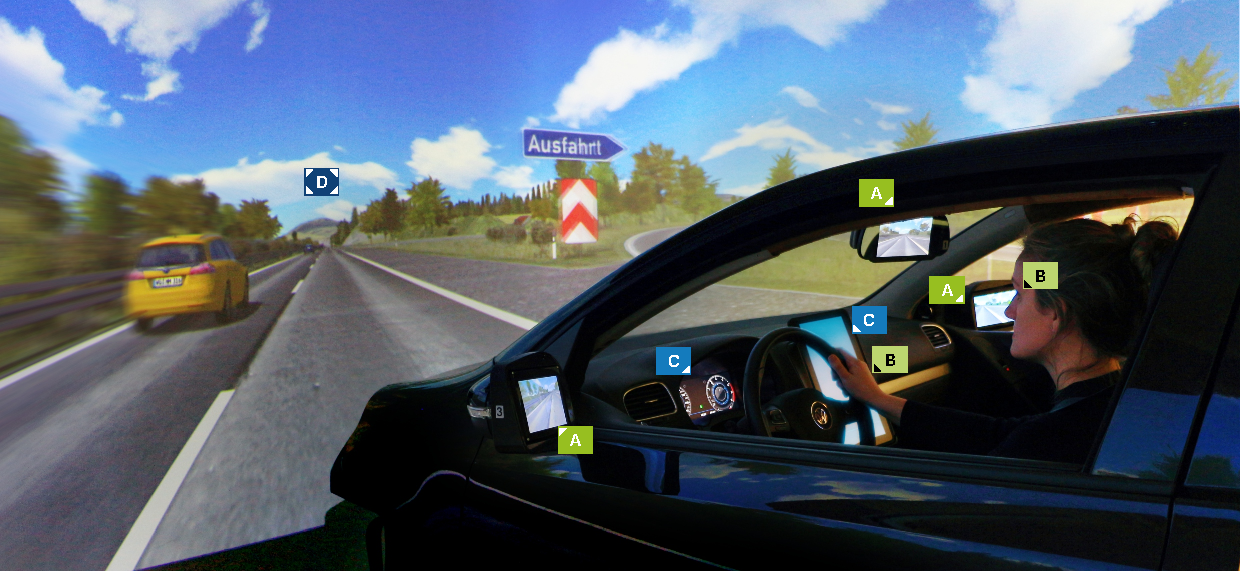
\includegraphics[width=\columnwidth]{content/caudri/images/ifab-sim1a}%
\end{nomargin} % nomargin muss vor der Caption enden, sonst ist die Caption zu breit
\caption{Der Fahrsimulator verfügt über digitale Rückspiegel (\textbf{A}) und die Möglichkeit, detailliert den Insassenzustand zu erheben (\textbf{B}), beispielsweise die Blickposition über Eye-Tracking oder Steuereingaben. Die vollständig digitalen Interieurdisplays (\textbf{C}) können nach Studienbedarf angepasst werden. Auf der 180°-Panoramaleinwand (\textbf{D}) können Fahrszenarien und Umgebungsbedingungen immersiv simuliert werden.}%
%
\end{figure*}

\newpage




Durch entsprechende frühzeitige Simulatorstudien kann sichergestellt werden, dass neue Funktionen von Anfang an menschengerecht entwickelt werden, was teuren Fehlentwicklungen vorbeugen kann. 


% Mit fquot könnt ihr ein abgesetztes Zitat aus dem Text einfügen. Ich würde es nicht zu häufig machen aber es kann Text etwas auflockern. Es ist okay, den Satz leicht anzupassen damit er besser für sich allein stehen kann.
\fquot{h}{Ein Fahrsimulator erlaubt die Erprobung verschiedenster Übergabeszenarien ohne Risiko und ohne, dass die technischen Fahrzeugfunktionen bereits real umgesetzt sein müssen.}{}

Simulatoren werden in verschiedenen Bereichen zum Training von bestimmten Fertigkeiten eingesetzt, z.B. bei der Ausbildung von Piloten mit Flugsimulatoren. Und auch im Bereich Gaming gibt es Ansätze, in denen ein Spielerlebnis mit der Vermittlung von Wissen oder Fähigkeiten verknüpft wird, sogenannte >>Serious Games<<. Die Forschung mit Fahrsimulatoren erhebt jedoch nicht den Anspruch, das Autofahren zu simulieren, sondern stelle eine >>fahrähnliche Aufgabe<< dar. Nachdem Erkenntnisse also zunächst risikofrei und kosteneffizient im Fahrsimulator erlangt werden, werden sie in der Regel im nächsten Schritt noch im Realverkehr erprobt, bevor sie im Fahrzeug umgesetzt werden.



\pagecolor{white} % Reset der (bisher schwarzen) Seitenfarbe



Der Fahrsimulator des IFAB am KIT besteht aus einem Golf-6 Fahrzeugelement, das beständig an die neuen Fahrzeuggenerationen angepasst wurde. Zuletzt wurde ein großer Mittelkonsolendisplay mit Touchfunktion verbaut, der die Bearbeitung von Nebenaufgaben oder Anzeige von Fahrzeugzustandsmeldungen erlaubt. Weitere Anzeigen, beispielsweise von Assistenzsystemen, sind im Tachodisplay möglich.

% Die Kontaktbox
\begin{wrapfigure}[20]{r}[2cm]{4cm}\vspace{-0.5cm}
\stylebox{4cm}{0.5cm}{Kontakt}{
\vspace{0.5em}
Institut für Arbeitswissenschaft \& Betriebsorganisation (IFAB)\\
am Karlsruher Institut für Technologie (KIT)

Engler-Bunte-Ring 4\\
Gebäude 40.29, Raum 006B\\
76131 Karlsruhe

Tel: +49 721-608-44250

Mail: info@ifab.kit.edu

Web: www.ifab.kit.edu\bigskip

\qrcode[height=1.5cm]{https://www.ifab.kit.edu/}
}
\end{wrapfigure}
Das Fahrzeugelement steht von einer speziellen 180°-Panoramaleinwand, auf die drei Beamer die Umgebung projizieren, die in der Software SILAB 7.1 der Firma WIVW GmbH simuliert wird. Der Blick zurück wird über Displays in den Außenspiegeln und im Innenspiegel ermöglicht. In Kombination führen die Anzeigen zu einem hohen Immersionserleben, man taucht also tief in die simulierte Umgebung ein.  Für eine möglichst detaillierte Erfassung des Fahrerverhaltens kann der Simulator mit weiteren Messsystemen kombiniert werden. Hierzu stehen dem IFAB beispielsweise Systeme zur Blickerfassung oder zur Messung physiologischer Parameter zur Verfügung.

Somit kann der Simulator am Standort Karlsruhe flexibel für eine weite Bandbreite an Studien im Bereich der Mensch-Maschine-Interaktion eingesetzt werden. Die technische Infrastruktur, sowie die Expertise zum Betrieb des Simulators und von Konzeption bis Durchführung gesamter Probandenstudien steht am IFAB für aktuelle und künftige Projekte zur Verfügung. 
\markEndOfContent % <- Das hier erzeugt die Box am Ende des Gesamtbeitrags.

\begin{figure*}[t]%
\begin{thinmargin} % Die thinmargin-Umgebung ragt in den Seitenrand-Bereich rein, aber nicht bis zur Kante. 
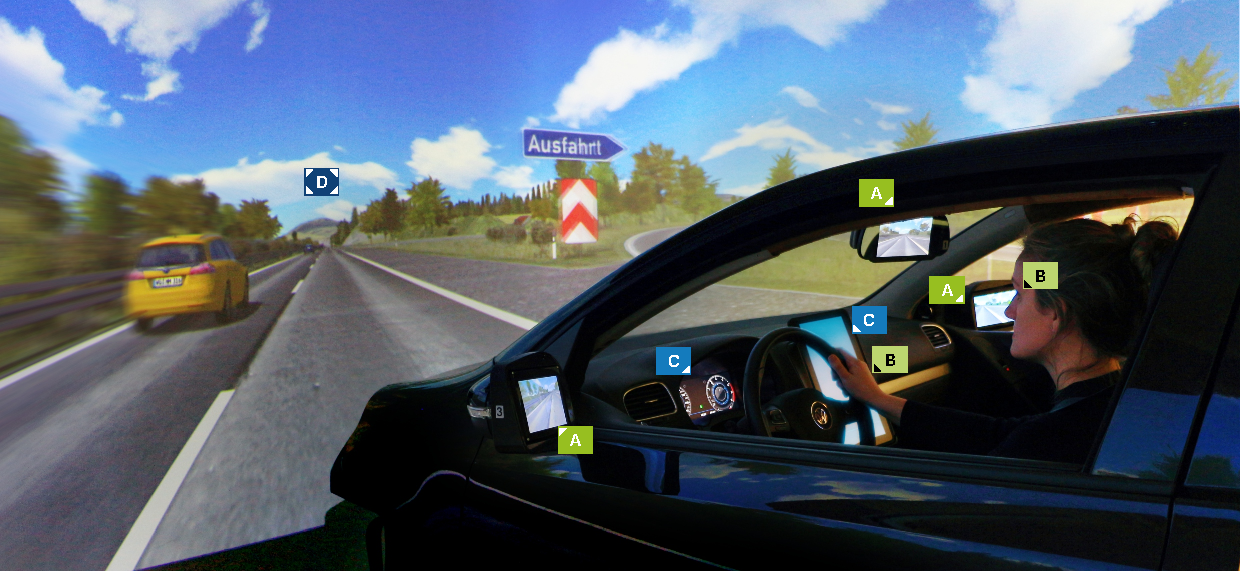
\includegraphics[width=\columnwidth]{content/caudri/images/ifab-sim1a}%

\caption{Die thinmargin-Umgebung ragt in den Seitenrand-Bereich rein, aber nicht bis zur Kante. }%
\end{thinmargin} % Bei thinmargin ist die Caption im thinmargin enthalten, sie wird also auch breiter.
\end{figure*}


\blindtext

\begin{figure*}[t]%
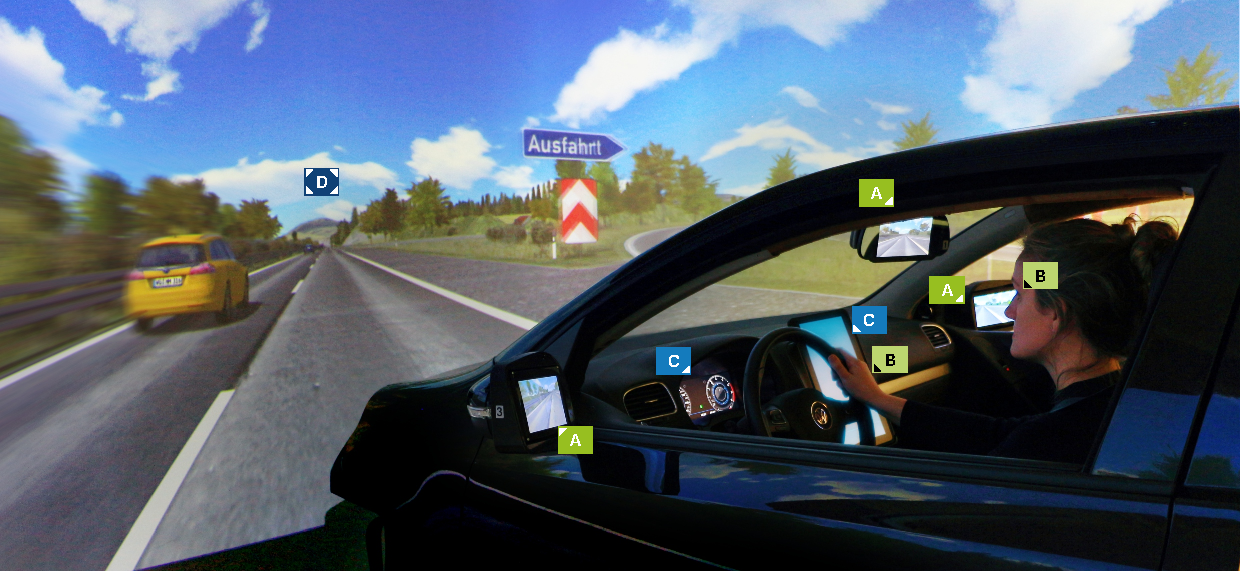
\includegraphics[width=\textwidth]{content/caudri/images/ifab-sim1a}%
\caption{Ohne thinmargin-Umgebung reichen Abbildungen nur über die Textspalten hinweg.}%
\end{figure*}



\Blindtext

% WICHTIG: Ich empfehle, als Bindestrich "= zu verwenden, wie im Beispiel unten, also Fahrzeug"=zu"=Fahrzeug"=Kommunikation zu schreiben. Dann verwendet LaTeX Silbentrennung für die Wörter "Fahrzeug" und "Kommunikation" (und "zu"). Wenn man stattdessen Fahrzeug-zu-Fahrzeug-Kommunikation schreibt, trennt LaTeX den Gesamtblock nur noch an den vorhandenen Bindestrichen, würde also das Wort "Kommunikation" bspw. nicht trennen.

\begin{figure*}[t]%
\stylebox{\textwidth}{0.5cm}{Wie funktioniert Fahrzeug"=zu"=Fahrzeug"=Kommunikation?}{

Infoboxen können den Text auch auflockern und wichtige Informationen absetzen. Sie können  \textbf{\color{colorKAMOLightBlue}einspaltig} oder \textbf{\color{colorKAMOLightGreen}zweispaltig} sein, je nachdem ob >>figure<< mit oder ohne Sternchen verwendet wird, und >>textwidth<< oder >>columnwidth<< als Breite angegeben wird.

Auch bei Infoboxen sollte man aber nicht zu viele platzieren. Ihr könnt ja mal schauen wie es bei der ersten Ausgabe aussieht.

Hier ist übrigens ein Beispiel für einen Literaturverweis \cite{ehrhardt2021gap}. Ihr müsst keine verwenden, aber wenn ihr wollt geht es so. Das Literaturverzeichnis wird >>pro Beitrag<< ausgegeben, es steht immer am Ende.
}
\end{figure*}

\Blindtext



\nocite{ziehn2023cooperative} % <- Dieser Literaturverweis erscheint nicht im Fließtext, wird aber trotzdem in das Literaturverzeichnis aufgenommen.

\printbibliography[heading=subbibliography]
